\documentclass{scrreprt}
\usepackage[english]{babel}
\usepackage[T1]{fontenc}
\usepackage{lmodern}
\usepackage{blindtext}
\usepackage[utf8]{inputenc}
\usepackage{siunitx} %For unit handling%
\renewcommand{\familydefault}{\sfdefault}
\newcommand{\unit}[1]{\ensuremath{\, \mathrm{#1}}}
\usepackage{amssymb, amsmath, cancel, ulem, graphicx, float, tabularx, multirow, bm}
\usepackage{amsmath}
\usepackage{caption}
\usepackage{subcaption}
\usepackage{tikz}
\newcommand*\circled[1]{\tikz[baseline=(char.base)]{
            \node[shape=circle,draw,inner sep=1pt] (char) {#1};}}
\renewcommand{\phi}{\varphi}

\setcounter{secnumdepth}{5}
\setcounter{tocdepth}{5}

\author{Urs Gerber\\09-921-156 \and Gian-Luca Mateo\\11-113-545}
\date{28th of March 2013}

\title{Forced Oscillation}
\subtitle{Practical course report}

\begin{document}

\maketitle

\tableofcontents
\newpage

\chapter{Experiment: Forced Oscillation}
\section{Introduction}
\subsection{Goal of the experiment}

\subsection{Theory}
\begin{equation}
J\cdot \ddot{\phi} = \sum_i M_i
\end{equation}
\subsubsection{Free damped oscillation}
\begin{equation}
M_R=-R\dot{\phi}
\end{equation}
\begin{equation}
J\ddot{\phi} + r \dot{\phi} + D \phi = 0
\end{equation}
The solution in case of weak damping is
\begin{equation}
\phi(t) = A e^{-\alpha t} \cos{\left(\omega t - \phi_0\right)}
\end{equation}

\section{Experiment setup and execution}
\subsection{Used materials}
The materials used in this experiment are the following:
\begin{itemize}
\item An hinged metal disc with an indicator at its top connected indirectly to an electric motor using a spring
\item A ring with a printed scale with greater inner radius than the metal disc's diameter
\item An eddy brake
\item A power supply with two outputs, one adjustable at 1-15V / 2A max and the other one fixed at 25V / 0.2A
\item A stopwatch
\item A multimeter (Model FLUKE 73 Multimeter)
\item six electric wires
\end{itemize}

\subsection{Assembly}

\begin{figure}[H]
	\centering
  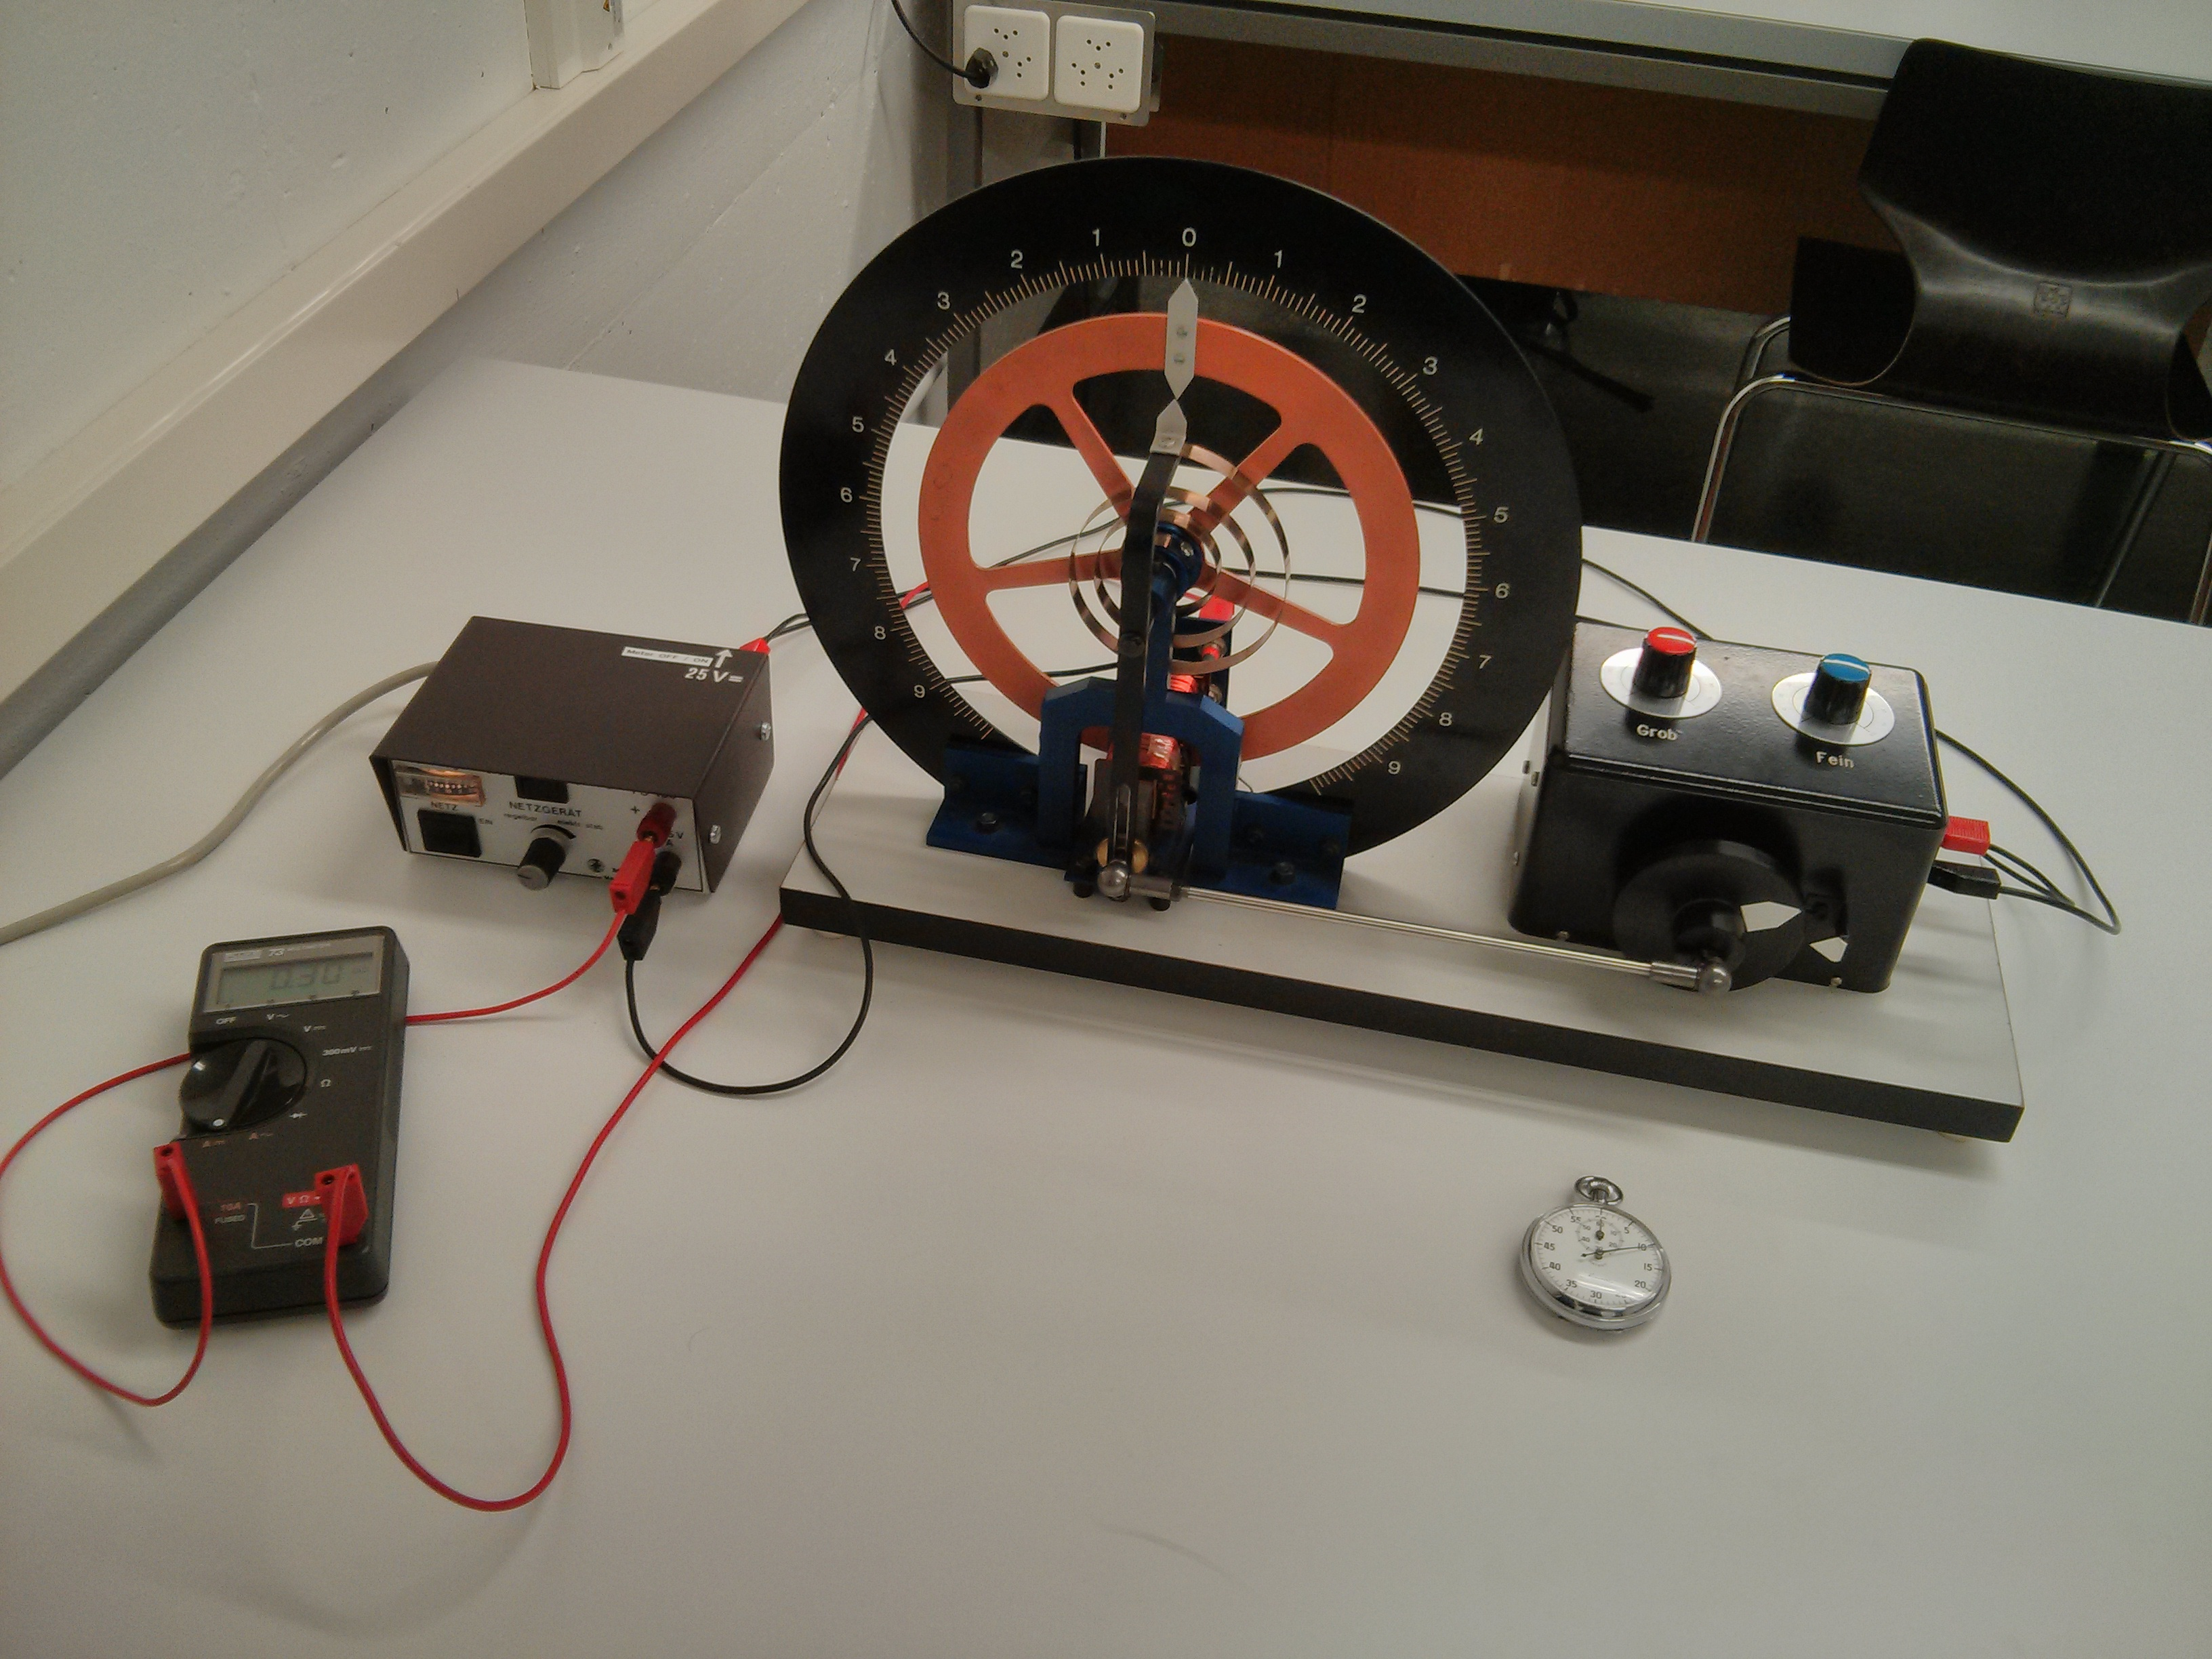
\includegraphics[width=0.9\textwidth]{img/assembly.jpg}
	\caption{The experiment assembly}
	\label{fig:assembly}
\end{figure}



\section{Measurements}

\section{Analysis and Discussion}

\section{Conclusion}


\begin{thebibliography}{9}

\bibitem{physcript13}
  Peter Wurz,
  \emph{Anleitung zum Physikpraktikum}
  FS2013

\end{thebibliography}

\end{document}
